%
% $RCSfile: interacting_systems.tex,v $
%
% Copyright (C) 2002-2008. Christian Heller.
%
% Permission is granted to copy, distribute and/or modify this document
% under the terms of the GNU Free Documentation License, Version 1.1 or
% any later version published by the Free Software Foundation; with no
% Invariant Sections, with no Front-Cover Texts and with no Back-Cover
% Texts. A copy of the license is included in the section entitled
% "GNU Free Documentation License".
%
% http://www.cybop.net
% - Cybernetics Oriented Programming -
%
% http://www.resmedicinae.org
% - Information in Medicine -
%
% Version: $Revision: 1.1 $ $Date: 2008-08-19 20:41:07 $ $Author: christian $
% Authors: Christian Heller <christian.heller@tuxtax.de>
%

\subsection{Interacting Systems}
\label{interacting_systems_heading}
\index{Interacting Systems}
\index{Information Technology Environment}
\index{IT Environment}
\index{Physical Architecture}
\index{Logical Architecture}
\index{Data Mapper}
\index{Data Transfer Object}
\index{DTO}
\index{Model View Controller}
\index{MVC}
\index{Communication Patterns}
\index{Conversion between Communication Models}
\index{Frontend Communication Model}
\index{Backend Communication Model}
\index{Remote Communication Model}
\index{Domain Communication Model}
\index{Persistence Layer}

Chapter \ref{physical_architecture_heading} introduced an example
\emph{Information Technology} (IT) environment (\emph{Physical Architecture}),
containing many interacting systems: server and client, local and remote, human
and artificial (figure \ref{communication_figure}). In (object oriented)
software design, special patterns are used to architect a system such that it
is able to communicate with other systems across various mechanisms
(\emph{Logical Architecture}). To these patterns count the \emph{Data Mapper},
\emph{Data Transfer Object} (DTO) and \emph{Model View Controller} (MVC)
(section \ref{pattern_heading}).

\begin{figure}[ht]
    \begin{center}
        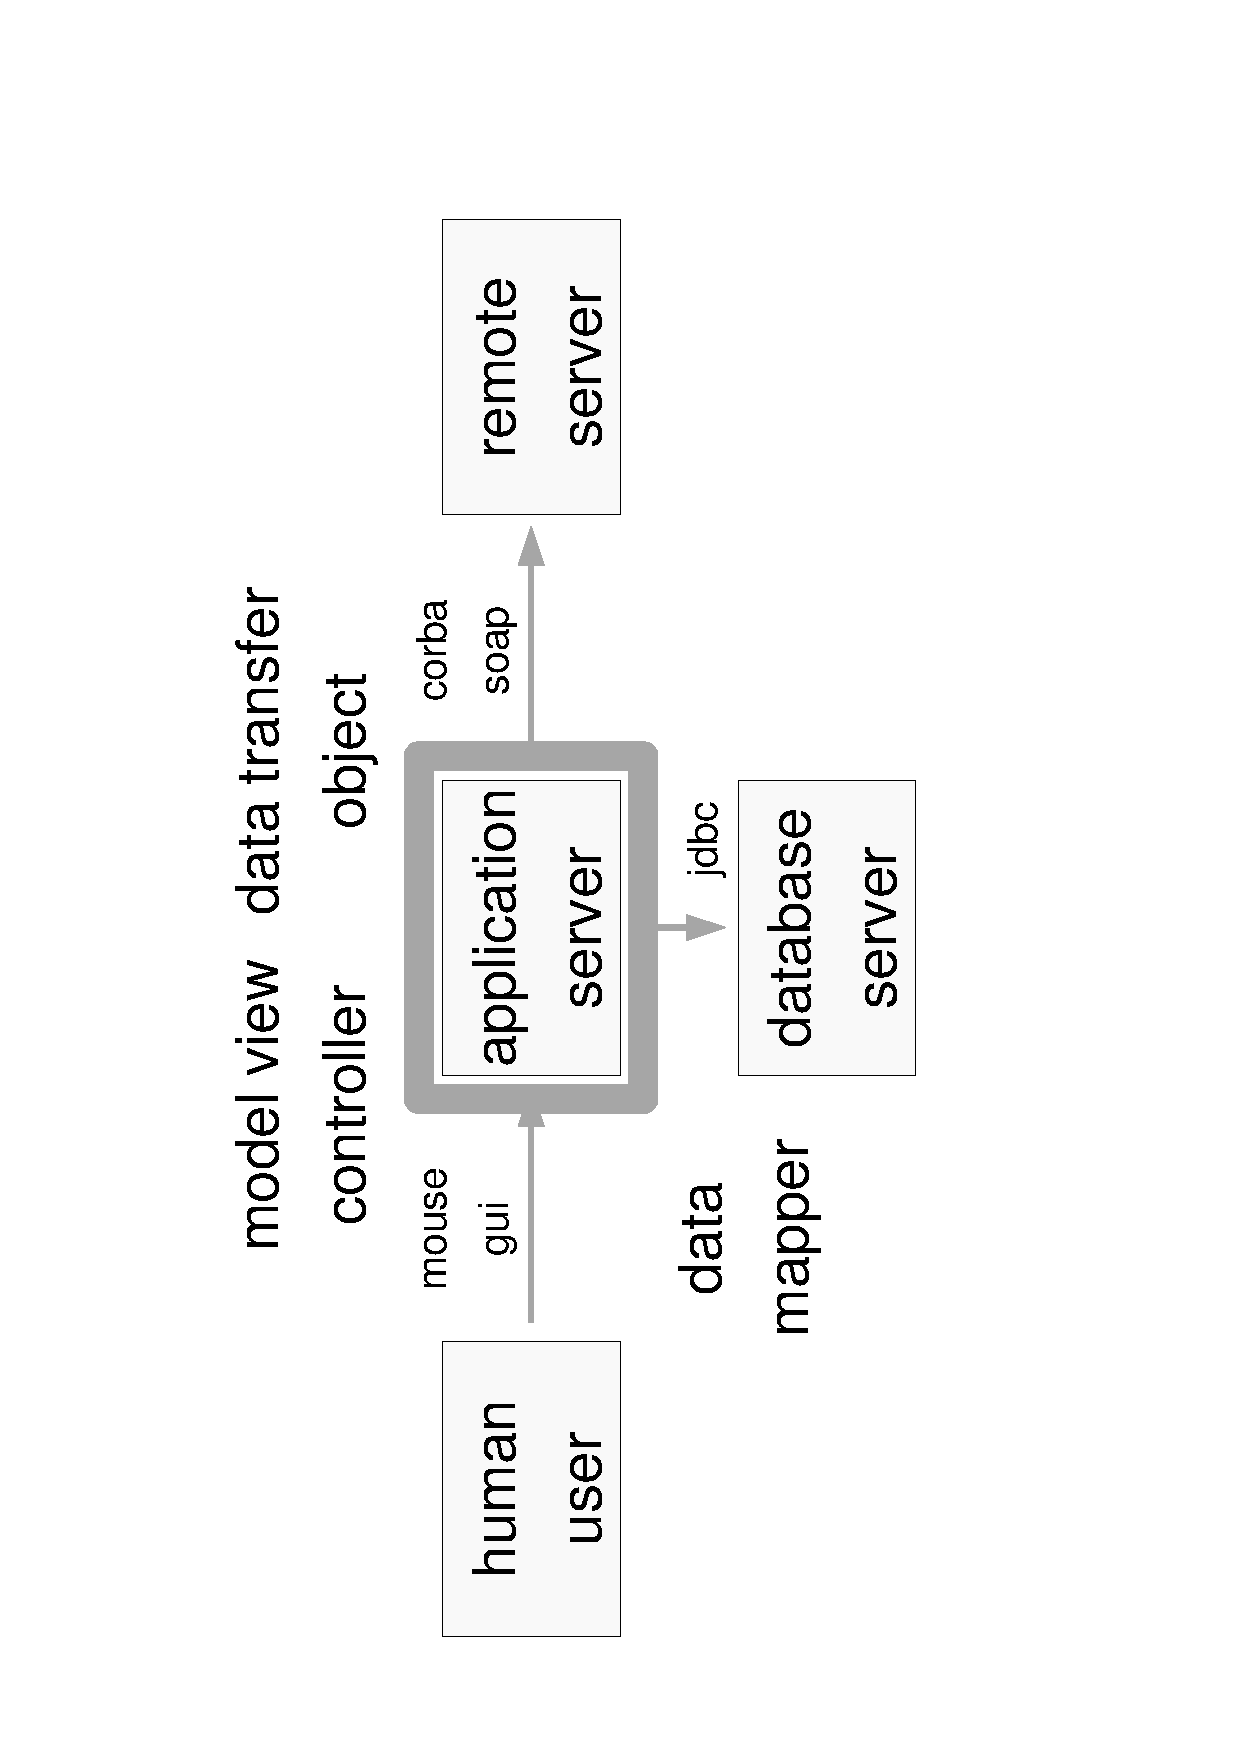
\includegraphics[scale=0.3,angle=-90]{graphic/communication.pdf}
        \caption{IT Environment with Server using Communication Patterns}
        \label{communication_figure}
    \end{center}
\end{figure}

Although software development has become a lot easier in the last decades, it is
still a big effort that should not be underestimated. One thing that application
developers have to care about much of their time is the \emph{Conversion}
between various kinds of (communication) models that a system has:

\begin{itemize}
    \item[-] Frontend (Communication with Human User)
    \item[-] Backend (Communication with Data Source)
    \item[-] Remote (Communication with Server)
    \item[-] Domain (Communication with own Knowledge)
\end{itemize}

The different mechanisms and patterns that have to be considered for such model
conversion often need to be implemented repeatedly, for each new application.
Some trials to unify all backend communication in a common \emph{Persistence Layer}
exist \cite{ambler}, but are remote- and frontend communication seldom considered
in a comparable way. Obviously, no current effort treats the frontend as just
another communication model that has to be \emph{sent} to the human user as
just another system.

The following sections will first reconsider three common communication
patterns, before embedding them into the classical model of logical system
layers (section \ref{layers_heading}). After that, a simplification is
suggested which finally leads to a new \emph{Translator Architecture} (first
introduced in \cite{hellerkunze}).
